\section*{Relationer i en retvinklet trekant}

For at bestemme sidelængderne og vinklerne i en retvinklet trekant bruger man nedenstående formler.

\begin{frm-thm}{Relationerne i den retvinklede trekant}

I den retvinklede trekant gælder følgende 3 relationer

$\cos(v) = \cfrac{\text{hosliggende katete}}{\text{hypotenusen}}$ \hspace*{2cm} $v = \cos^{-1}\left(\cfrac{\text{hosliggende katete}}{\text{hypotenusen}}\right)$

$\sin(v) = \cfrac{\text{modstående katete}}{\text{hypotenusen}}$ \hspace*{2cm} $v = \sin^{-1}\left(\cfrac{\text{modstående katete}}{\text{hypotenusen}}\right)$

$\tan(v) = \cfrac{\text{modstående katete}}{\text{hosliggende katete}}$ \hspace*{2cm} $v = \tan^{-1}\left(\cfrac{\text{modstående katete}}{\text{hosliggende katete}}\right)$

\end{frm-thm}

Hvis vi kender 1 vinkel og 1 sidelængde kan vi ud fra relationerne i den retvinklede trekant bestemme de resterende sidelængder. Kender vi ingen vinkler men 2 sidelængder kan vi bestemme de resterende vinkler.

Vi betragter nu følgende 2 eksempler

\textbf{Eksempel 1: Beregning af sidelængde}

Vi er givet følgende retvinklede trekant

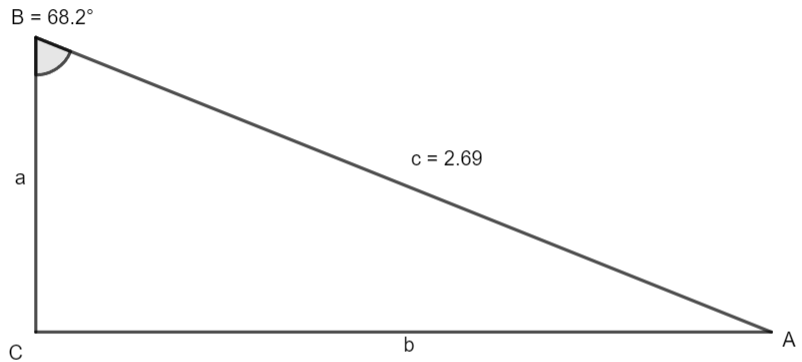
\includegraphics[scale=0.7]{img_1}

og bliver bedt om at bestemme længden af siden b.

For at bestemme længden af siden b skal vi først finde ud af hvilken af de 3 relationer vi skal bruge. Hvis vi kigger på trekanten fra vinkel B som vi kender, er siden b den modstående katete. Desuden kender vi længden af siden c som er trekantens hypotenuse. Vi finder nu den relation som indeholder den modstående katete og hypotenusen. Denne relation er $\sin(v) = \cfrac{\text{modstående katete}}{\text{hypotenusen}} $

Vi indsætter nu de kendte værdier og isolerer siden b.

\begin{align*}
&\sin(B) = \frac{b}{c}\\
\Updownarrow \hspace*{2mm} &\\
&\sin(68.2^{\circ}) = \frac{b}{2.69} && B = 68.2^{\circ}, c = 2.69\\
\Updownarrow \hspace*{2mm} &\\
&\sin(68.2^{\circ}) \cdot 2.69 = b && \text{flytter 2.69 over på den anden side} \\
\Updownarrow \hspace*{2mm} &\\
&b = \sin(68.2^{\circ}) \cdot 2.69 && \text{bytter om på højre og venstre side}\\
\Updownarrow \hspace*{2mm} &\\
&b = 2.5
\end{align*}

Vi får dermed længden af side b til $b = 2.5$

\textbf{Eksempel 2: Beregning af vinkel}

Vi er givet følgende retvinklede trekant

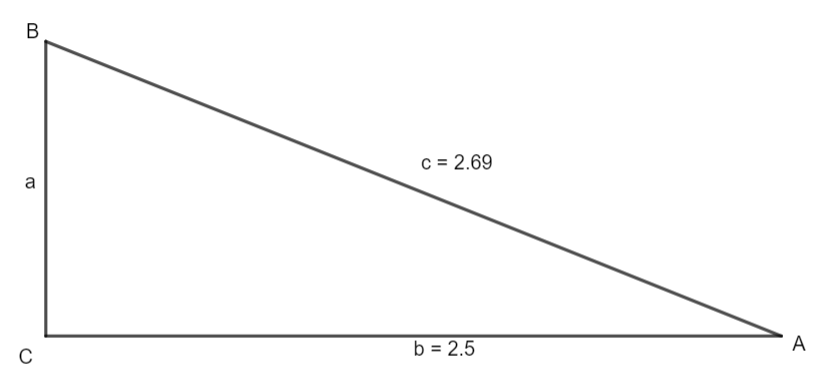
\includegraphics[scale=0.7]{img_2}

og bliver bedt om at bestemme vinklen A.

For at bestemme Vinklen A skal vi først finde ud af hvilken af de 3 relationer vi skal bruge. Hvis vi kigger på trekanten fra vinkel A er siden b, som vi kender, den hosliggende katete og siden c, som vi kender, hypotenusen. Vi finder nu den relation som indeholder den hosliggende katete og hypotenusen. Denne relation er $\cos(v) = \cfrac{\text{hosliggende katete}}{\text{hypotenusen}}$ og den tilsvarende formel for at finde vinklen er $v = \cos^{-1}\left(\cfrac{\text{hosliggende katete}}{\text{hypotenusen}}\right) $. Vi indsætter nu de kendte værdier og får

\begin{align*}
&v = \cos^{-1}\left(\frac{\text{hosliggende katete}}{\text{hypotenusen}}\right)\\
\Updownarrow \hspace*{2mm} &\\
&A = \cos^{-1}\left(\frac{b}{c}\right)\\
\Updownarrow \hspace*{2mm} &\\
&A = \cos^{-1}\left(\frac{2.5}{2.69}\right)\\
\Updownarrow \hspace*{2mm} &\\
&A = 21.66^{\circ}
\end{align*}

\section*{Opgaver}

\textbf{1.}
Bestem vinkel A i følgende trekant

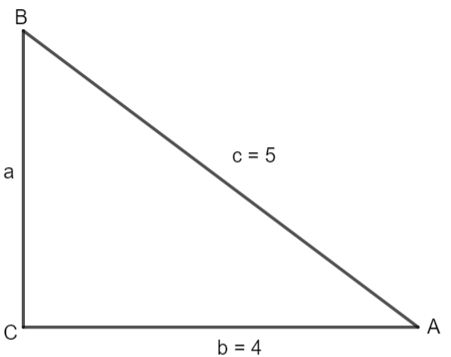
\includegraphics[scale=0.7]{img_3}

\textbf{2.}
Bestem vinkel B i følgende trekant

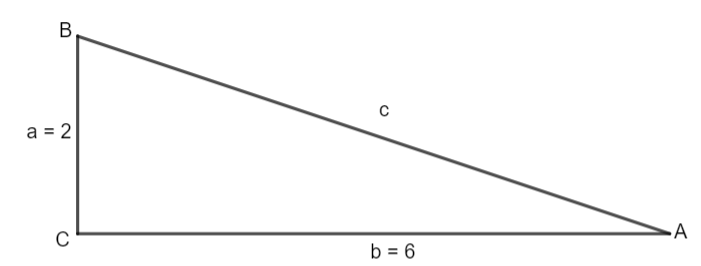
\includegraphics[scale=0.7]{img_5}

\textbf{3.}
Bestem sidelængde b i følgende trekant

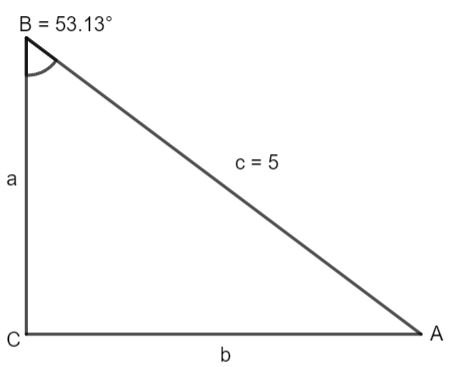
\includegraphics[scale=0.7]{img_4}

\textbf{4.}
Bestem sidelængde c i følgende trekant

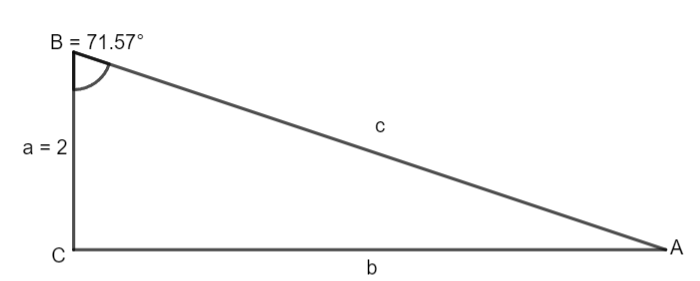
\includegraphics[scale=0.7]{img_6}


\newpage

\section*{Facit}

\textbf{1.} $A = 36.87^{\circ}$

\textbf{2.} $B = 71.57^{\circ}$

\textbf{3.} $b = 4$

\textbf{4.} $c = 6.32$